\documentclass{article}

\usepackage{hyperref}
\usepackage[T1]{fontenc}
\usepackage{graphicx}
\usepackage{float}
\usepackage[utf8]{inputenc}
\usepackage{amsmath}
\usepackage{amsfonts}


\title{%
Laboratorium 11\\
  \huge Optymalizacja}
\author{Mateusz Król}
\date{15/06/2024 r.}

\begin{document}
\maketitle

 
\section*{Zadanie 1.}
\textbf{Wyznacz punkty krytyczne każdej z poniższych funkcji.
Scharakteryzuj każdy znaleziony punkt jako minimum, maksimum lub punkt siodłowy.
Dla każdej funkcji zbadaj, czy posiada minimum globalne lub maksimum globalne na zbiorze $\mathbb{R}$.}
$$f_1(x, y) = x^2 - 4xy + y^2$$
$$f_2(x, y) = x^4 - 4xy + y^4$$
$$f_3(x, y) = 2x^3 - 3x^2 -6xy(x-y-1)$$
$$f_4(x, y) = (x-y)^4 + x^2 - y^2 - 2x + 2y +1$$
\\\\
Dla funkcji $f_1$:
$$\frac{\partial f_1}{\partial x} = 2x-4y = 0$$
$$\frac{\partial f_1}{\partial y} = -4x+2y = 0$$
Punkty krytyczne:
$$(x, y) = (0, 0)$$
Macierz Hessego:
$$H = \begin{bmatrix}
  2 & -4 \\
  -4 & 2 
\end{bmatrix}$$
$$det(H) = -12 < 0$$
Punkt $(0, 0)$ jest punktem siodłowym. \\


Dla funkcji $f_2$:
$$\frac{\partial f_2}{\partial x} = 4x^3-4y = 0$$
$$\frac{\partial f_2}{\partial y} = -4x+4y^3 = 0$$
Punkty krytyczne:
$$(x, y) = (0, 0), (1, 1), (-1, -1)$$
Macierz Hessego:
$$H = \begin{bmatrix}
  12x^2 & -4 \\
  -4 & 12y^2
\end{bmatrix}$$
$$det(H(0, 0)) = -16 < 0$$
Punkt $(0, 0)$ jest punktem siodłowym.
$$det(H(1, 1)) = 128 > 0$$

$$\frac{\partial^2 f_1}{\partial x^2}(1, 1) = 12 > 0$$
Punkt $(1, 1)$ jest minimum lokalnym.

$$det(H(-1, -1)) = 128 > 0$$
$$\frac{\partial^2 f_2}{\partial x^2}(-1, -1) = 12 > 0$$
Punkt $(-1, -1)$ jest minimum lokalnym. \\

Dla funkcji $f_3$:
$$\frac{\partial f_3}{\partial x} = 6x^2-6x-12xy+6y^2+6y = 0$$
$$\frac{\partial f_3}{\partial y} = -6x^2+6xy+6x = 0$$
Punkty krytyczne:
$$(x, y) = (0, 0), (-1, -1), (0, -1), (1, 0) $$
Macierz Hessego:
$$H = \begin{bmatrix}
  12x-6-12y & -12x+12y+6 \\
  -12x+12y+6 & 12x
\end{bmatrix}$$

$$det(H(0, 0)) = -36 < 0$$
Punkt $(0, 0)$ jest punktem siodłowym. \\

$$det(H(-1, -1)) = 36 > 0$$
$$\frac{\partial^2 f_3}{\partial x^2}(-1, -1) = -6 < 0$$
Punkt $(-1, -1)$ jest maksimum lokalnym  \\

$$det(H(1, 0)) = 36 > 0$$
$$\frac{\partial^2 f_3}{\partial x^2}(1, 0) = 6 > 0$$
Punkt $(1, 0)$ jest minimum lokalnym. \\

$$det(H(0, -1)) = -36 < 0$$
Punkt $(0, -1)$ jest punktem siodłowym. \\


Dla funkcji $f_4$:
$$\frac{\partial f_4}{\partial x} = 4(x-y)^3 + 2x - 2 = 0$$
$$\frac{\partial f_4}{\partial y} = -4(x-y)^3 -2y + 2 = 0$$
Punkty krytyczne:
$$(x, y) = (0, 0)$$

Macierz Hessego:
$$H = \begin{bmatrix}
  -12(x-y)^2 + 2 & -12(x-y)^2 \\
  -12(x-y)^2 & 12(x-y)^2-2 
\end{bmatrix}$$
$$det(H(1, 1)) = -4 < 0$$
Punkt $(1, 1)$ jest punktem siodłowym.



\section*{Zadanie 2.}
\textbf{Należy wyznaczyć najkrótszą ścieżkę robota pomiędzy dwoma punktami
$x^{(0)}$ i $x^{(n)}$. \\
Problemem są przeszkody usytuowane na trasie robota, których
należy unikać.\\
Zadanie polega na minimalizacji funkcja kosztu, która sprowadza
problem nieliniowej optymalizacji z ograniczeniami do problemu nieograniczonej
optymalizacji.}
\\\\

Algorytm największego spadku z przeszukiwaniem liniowym (ang. \textit{Gradient Descent with Line Search})
iteracyjnie znajduje minimum funkcji celu poprzez poruszanie się w kierunku przeciwnym do
obliczonego na podstawie gradientu funkcji. Do przeszukiwania liniowego wykorzystuję metodę złotego podziału
(ang. \textit{Golden Section Search}), która znajduje optymalny krok $\alpha$ wzdłuż kierunku gradientu.
\\\\
Kroki algorytmu:
\begin{itemize}
  \item punkty początkowe: $x$\\
  \item przedział poszukiwań dla $\alpha$ \\
  \item iteracyjnie: obliczenie gradientu, znalezienie optymalnego $\alpha$ dla funkcji $F(x_{k} - \alpha \cdot grad(F(x_k)))$
  , aktualizacja $x_{k+1} = x_k - \alpha \cdot grad(F(x_k))$ \\
\end{itemize}

\null\quad
Pięcio krotnie wylosowałem początkowe wartości $x$ z rozkładu jednostajnego z przedziału
$(0; 20)$.\\
\null\quad
Poniżej znajdują się wykresy odpowiadające końcowym wartościom $x$, czyli ścieżce 
\textit{wybranej} przez robota: \\

\begin{figure}[H]
  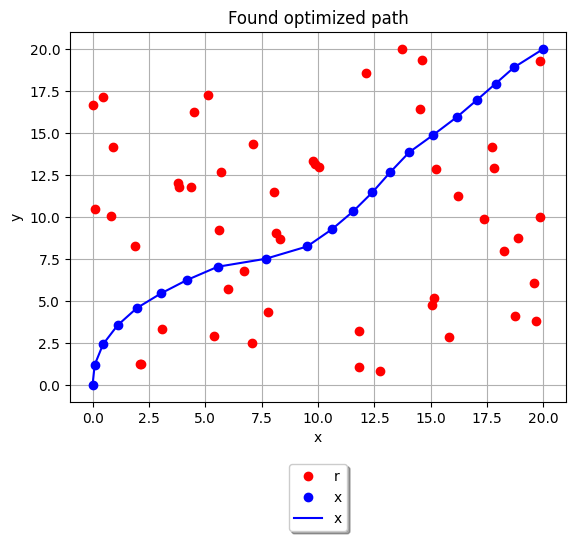
\includegraphics[width=\linewidth]{figures/1.png}
\end{figure}

\begin{figure}[H]
  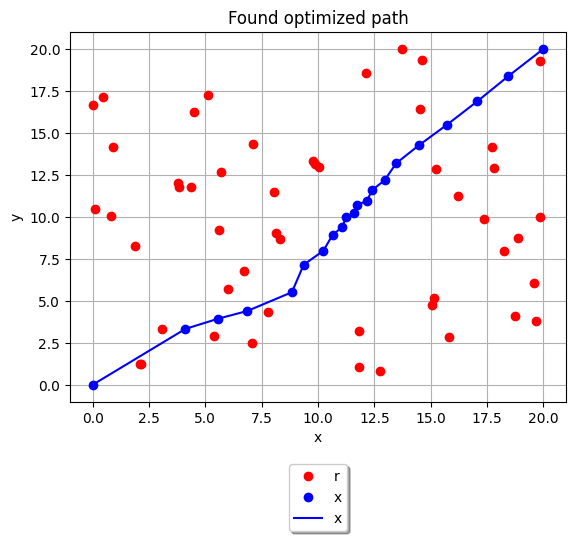
\includegraphics[width=\linewidth]{figures/2.png}
\end{figure}

\begin{figure}[H]
  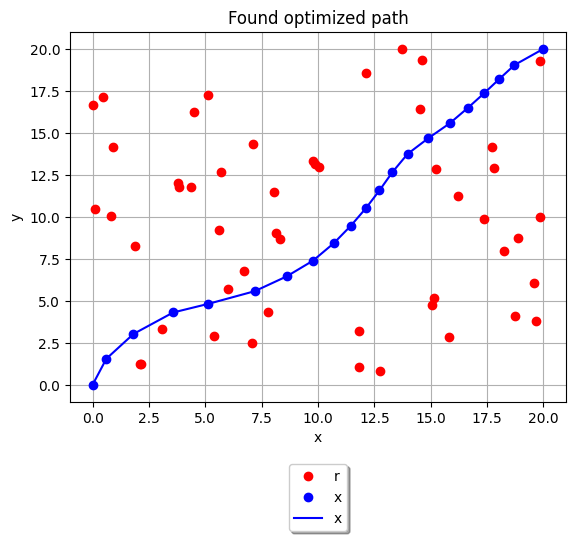
\includegraphics[width=\linewidth]{figures/3.png}
\end{figure}

\begin{figure}[H]
  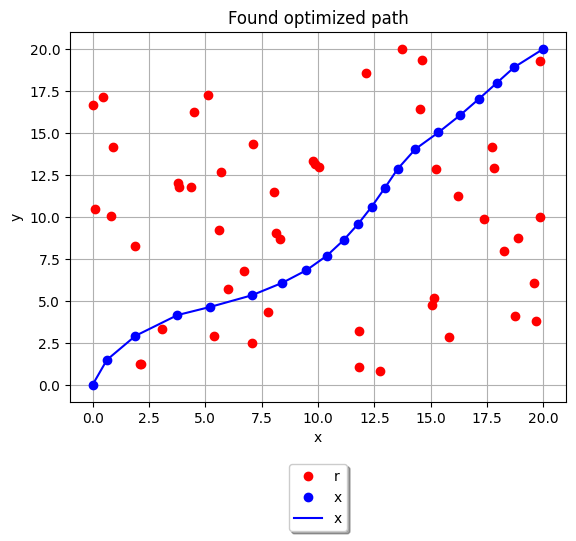
\includegraphics[width=\linewidth]{figures/4.png}
\end{figure}

\begin{figure}[H]
  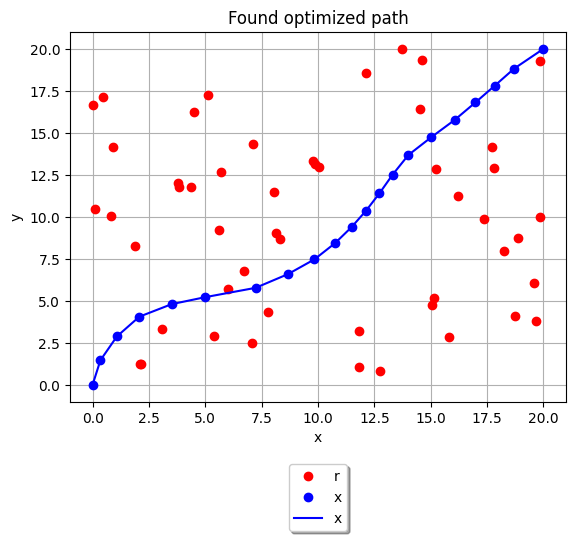
\includegraphics[width=\linewidth]{figures/5.png}
\end{figure}

\newpage
Poniżej znajduje się wykres wartości funkcji kosztu $F$ w zależności od dotychczasowej
liczby iteracji:

\begin{figure}[H]
  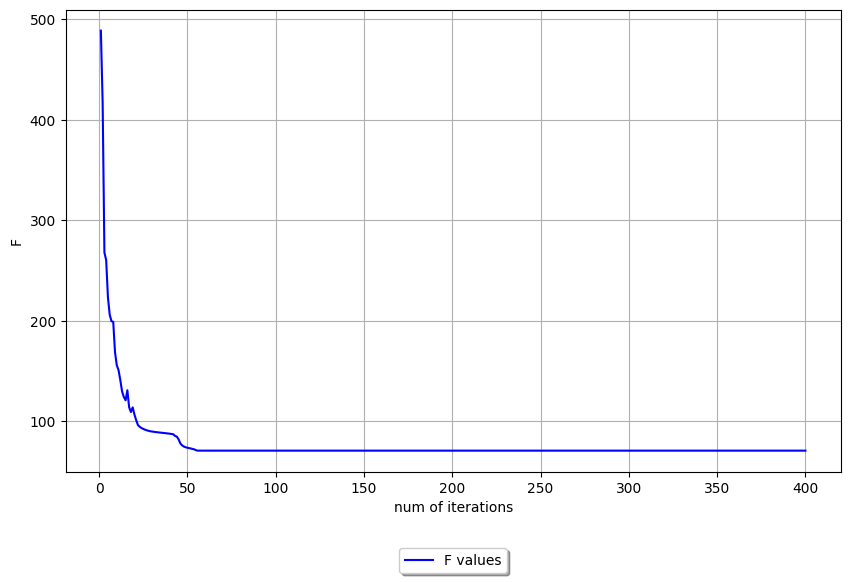
\includegraphics[width=\linewidth]{figures/F.png}
\end{figure}

Wartości funkcji $F$ bardzo szybko maleją, wydają się zbiegać do wartości $\approx 70.78$.

\section*{Wnioski}
\null\quad
W \textbf{Zadaniu 1.}: \\
Funkcja $f_1$ nie posiada globalnego minimum ani maksimum na zbiorze $\mathbb{R}$,
gdyż jej granice niewłaściwe są rozbieżne (funkcja może rosnąć lub maleć bez ograniczeń). \\
Funkcja $f_2$ nie posiada globalnego maksimum na zbiorze $\mathbb{R}$. Globalne minimum wynosi $-2$ i 
jest przyjmowane w punktach $(1, 1)$ oraz $(-1, -1)$. \\
Funkcja $f_3$ nie posiada globalnego minimum ani maksimum na zbiorze $\mathbb{R}$,
gdyż jej granice niewłaściwe są rozbieżne (funkcja może rosnąć lub maleć bez ograniczeń). \\
Funkcja $f_4$ nie posiada globalnego minimum ani maksimum na zbiorze $\mathbb{R}$,
gdyż jej granice niewłaściwe są rozbieżne (funkcja może rosnąć lub maleć bez ograniczeń). \\
\null\quad
W \textbf{Zadaniu 2.}: \\
Wykorzystana metoda okazała się być skuteczna w zaproponowanym zastosowaniu - znajdywaniu przez robota
ścieżki między przeszkodami. \\
Spadek wzdłuż gradientu posiada różne wady, m.in. nie gwarantuje znalezienia maksimum globalnego, ale
okazał się być odpowiedni przy wybranej konfiguracji problemu. \\
Algorytm szukania ścieżki można by zmodyfikować: założyc stały parametr $\alpha$, co zmniejszyłoby
złożoność obliczeniową problemu.





\end{document}